%% =====================================================================
%%  The Last Scarcity
%%  Meaning and measurement after machines saturate the Gaokao
%%
%%  Build:  pdflatex main.tex  (run twice)   |  arXiv-ready, TeX Live
%% =====================================================================
\pdfoutput=1
\documentclass[11pt]{article}

\usepackage[margin=1in]{geometry}
\usepackage[T1]{fontenc}
\usepackage[utf8]{inputenc}
\usepackage{lmodern}
\usepackage{microtype}
\usepackage{amsmath,amssymb}
\usepackage{amsthm}
\usepackage{booktabs}
\usepackage{graphicx}
\usepackage{caption}
\usepackage{enumitem}
\usepackage{xcolor}
\usepackage[numbers,sort&compress]{natbib}
\usepackage[colorlinks=true,linkcolor=black,citecolor=black,
            urlcolor={blue!35!black}]{hyperref}
\usepackage{xurl}

\captionsetup{font=small,labelfont=bf,width=0.94\textwidth}
\setlist{itemsep=2pt,topsep=4pt}
\emergencystretch=1.5em

\theoremstyle{plain}
\newtheorem{proposition}{Proposition}
\newtheorem*{relocationcor}{Corollary}

\hypersetup{
  pdftitle={The Last Scarcity: Meaning and Measurement After Machines
            Saturate the Gaokao},
  pdfauthor={Xinhao Zheng},
  pdfsubject={AI agent evaluation; benchmark saturation; measurement},
}

\newcommand{\Q}[1]{Q#1}

\title{\textbf{The Last Scarcity:\\[3pt]
  Meaning and Measurement After Machines\\
  Saturate the Gaokao}}
\author{%
  Xinhao Zheng\thanks{Correspondence: \texttt{xinhaozheng.vx@outlook.com}.
    Code and data:
    \url{https://github.com/xinhao-zheng/ncee-2026-math-agent-eval}.}\\[2pt]
  \small Independent Researcher}
\date{11 June 2026}

\begin{document}
\maketitle

\begin{abstract}
\noindent
Benchmarks are instruments, and instruments price scarcity. Days after
its public release, we administered the mathematics paper of the 2026
Chinese National College Entrance Examination (Gaokao; New Curriculum
Paper~I: 19 items, 150 points) to ten commercially deployed AI agents
from five model families under closed-book isolation: agents saw the item
stems and a submission template; keys, rubrics, and all prior submissions
were withheld. Five agents spanning three vendors returned a
perfect $150/150$ (cohort mean $137.8$, median $145$); the fastest perfect
paper took $4$\,min~$24$\,s. Residual errors concentrate where solutions
require global case analysis or extremal certification rather than
computation. On the eight conclusions where the answer key circulating
online fails independent verification, the cohort sided almost without
exception with the verified values: these systems derive; they do not
recall. Wall-clock time is decoupled from score. The
examination has saturated as a measure of machine mathematics---but the
deeper casualty is the proxy it rested on. We read the collapse causally:
a score is a signal worth the cost of producing it, and within the
measured range that cost has fallen to minutes; a measurement outcome has
meaning for a system only insofar as the system's future can still depend
on it, and for frozen-weight systems no such dependence exists. When
solving becomes abundant and consequence-free, scores stop pricing
excellence; what remains scarce, and therefore measurable, and therefore
meaningful, is what still carries irreversible cost and consequence:
wanting, posing, adjudicating, staking. Machines have outcomes. Humans
have fates.
\end{abstract}

\paragraph*{Keywords.} agent evaluation; benchmark saturation; Gaokao;
data contamination; measurement; meaning.

\section{Introduction}

An examination is an instrument calibrated to a population, and a price
list for what that population holds scarce. The Gaokao mathematics paper
is the largest such instrument on earth: each June it spreads roughly
thirteen million candidates across 150 points, and the resulting order is
exchanged for universities, cities, trajectories---for lives. Its
authority rests on a proxy so old that it is rarely stated: that
performance on well-posed problems under sealed conditions indexes a
scarce and consequential human excellence---in psychometric terms, a
validity claim \citep{cronbach1955construct}. Administering the instrument to
a new kind of examinee tests the proxy, not merely the examinee. If the
newcomers collapse the score distribution, the paper has not become
easier; the excellence it prices has stopped being scarce. This article
reports such a collapse, observed within days of the instrument's first
use.

A collapse is informative only if the examinee cannot have memorized the
instrument. Evaluations built on past papers are compromised by
construction: stems, keys, and worked solutions saturate training corpora
\citep{carlini2023quantifying,zhang2024careful}.
A freshly administered paper opens a brief contamination-resistant
window---stems public for days, solutions scarce and unstable. The 2026
administration supplied the window and, unplanned, a control. Re-deriving
every answer independently, we found that the answer key circulating
online---the very artifact a memorizing system would absorb---fails
verification on eight conclusions (Appendix~\ref{app:errata}). A system
that recalls and a system that derives are indistinguishable on the
correct conclusions; they separate exactly on the wrong eight. Where
black-box contamination tests must infer exposure from likelihood
statistics \citep{oren2024proving}, a defective key supplies a behavioral
discriminant.

The Gaokao is not new to machine evaluation; the window is. AGIEval and
GAOKAO-Bench administer past papers
\citep{zhong2023agieval,zhang2023gaokaobench}, squarely inside the
contaminated regime; GAOKAO-Eval moved to the fresh 2024 paper to ask
whether high scores track human-aligned ability \citep{lei2024gaokaoeval};
live benchmarks institutionalize recency itself
\citep{white2025livebench,balunovic2025matharena}; fresh olympiads have
been graded within hours of release \citep{petrov2025proof}. Mathematics
benchmarks at large trace a single life cycle---posed, climbed, saturated,
succeeded by something harder: GSM8K, MATH, FrontierMath, Humanity's Last
Exam \citep{cobbe2021gsm8k,hendrycks2021math,glazer2024frontiermath,
phan2025hle}. This article does not add a rung to the ladder. It reports
from one at the moment of saturation and asks what the saturation itself
measures.

The design is deliberately simple---a controlled snapshot, not a
leaderboard. We transcribed New Curriculum Paper~I into bilingual,
machine-readable form, placed ten agents from five families one at a time
in an isolated workspace containing only the stems and a submission
template, recorded shell-clock timestamps, and scored every submission
against the errata-verified key under a fixed rubric. One run per agent;
no resampling; every artifact frozen into an immutable ledger and
released.

The article contributes four things: a minimal, reproducible
closed-book protocol for administering human examinations to AI
agents---isolation surfaces, prompts, shell-clock timing, immutable
ledger (\S\ref{sec:method}); a complete saturation datapoint---ten
agents, five families, half the cohort at ceiling, with the full
section- and item-level failure structure (\S\ref{sec:results}); an
unplanned recall-versus-derivation control built from the eight errors
of the circulating key (\S\ref{sec:results}, F4); and a causal account
of the collapse---three general propositions on exhaustion, repricing,
and meaning, instantiated by this run yet independent of this exam,
this cohort, and this year, together with the measurement program they
imply (\S\ref{sec:discussion}).

\section{Method}
\label{sec:method}

\subsection{Instrument}

The paper comprises 19 items worth 150 points
(Table~\ref{tab:instrument}). Stems were transcribed into bilingual
(Chinese--English) Markdown with all mathematics in LaTeX; the single
diagram (\Q{15}) is embedded as TikZ source, so agents read a symbolic
rather than raster figure. Every answer was re-derived independently; we
treat no circulating key as authoritative. The eight circulated
conclusions that fail verification are listed in
Appendix~\ref{app:errata}, and the verified values govern
scoring---circulated-but-wrong variants earn no credit.

\begin{table}[t]
  \centering\small
  \caption{Instrument structure and scoring rules.}
  \label{tab:instrument}
  \begin{tabular}{@{}llrl@{}}
    \toprule
    Section & Items & Points & Rule \\
    \midrule
    Single choice   & \Q{1}--\Q{8}   & 40 & 5 each; exactly one correct option \\
    Multiple choice & \Q{9}--\Q{11}  & 18 & 6 each: all correct 6 / proper subset 3 / any wrong 0 \\
    Fill-in         & \Q{12}--\Q{14} & 15 & 5 each; equivalent forms accepted; \Q{13} split $2.5+2.5$ \\
    Free response   & \Q{15}--\Q{19} & 77 & $13+15+15+17+17$; partial credit per rubric \\
    \bottomrule
  \end{tabular}
\end{table}

\subsection{Isolation protocol}

Each evaluation runs in four phases. \emph{Prepare}: the key, rubric,
results ledger, manuscript, and tooling are removed from the
subject-visible workspace; the submissions directory is cleared except for
a template. \emph{Exam}: the subject agent may read exactly three
files---the protocol README, the stems, and the template; it must obtain
\texttt{started\_at} from the shell clock before reading the stems, answer
all 19 items, and write a single Markdown submission whose front matter
records timestamps, duration, and model identity. \emph{Score}: key and
rubric are restored and a scorer grades the submission item by item.
\emph{Publish}: submissions, reports, and a manifest are frozen under
\texttt{results/<run\_id>/}. No agent ever sees a key, a rubric, or
another agent's output.

\subsection{Cohort}

Ten agents from five families ran on 10 June 2026 in the same IDE-based
harness (Cursor): Anthropic Claude ($n{=}3$), OpenAI GPT ($n{=}3$), Google
Gemini ($n{=}2$), Moonshot AI Kimi ($n{=}1$), and Cursor Composer
($n{=}1$). All ran with provider defaults; wherever the harness exposed a
reasoning-effort selector, it was set to \emph{medium}. The remaining
toggles---extended thinking, fast variants, ``Max Mode''---follow the
harness's model selection and are listed in Table~\ref{tab:results}.
Three submissions self-report a higher effort level (high or max) in
their front matter; the ledger preserves those records verbatim, and the
operator setting governs the reporting here. Wall-clock duration spans
first read to final save and includes tool orchestration and file I/O: it
is a property of the deployment, not of the model alone.

\subsection{Scoring}

A single scorer agent (Composer~2.5 Fast---itself a cohort member; we
disclose the conflict) graded all ten submissions against the verified key
and the published rubric. Objective items (73 of 150 points) are
mechanically checkable; free-response credit follows the rubric's step
breakdown. All ten score reports, including per-item match notes, are
released for audit.

\section{Results}
\label{sec:results}

\begin{table}[t]
  \centering\small
  \setlength{\tabcolsep}{4.6pt}
  \caption{Cohort, configuration, wall-clock time, and scores.
    SC/MC/FI/FR = single choice (40), multiple choice (18), fill-in (15),
    free response (77). Configuration lists variant toggles per the
    harness model selection; reasoning effort was operator-set to
    \emph{medium} wherever a selector existed (three submissions
    self-report otherwise; the ledger preserves those records). Time is
    m:ss on the shell clock.}
  \label{tab:results}
  \begin{tabular}{@{}llllrrrrr@{}}
    \toprule
    Model & Family & Configuration & Time & SC & MC & FI & FR & Total \\
    \midrule
    Fable 5           & Claude   & thinking           & 12:30 & 40 & 18 & 15 & 77 & \textbf{150} \\
    Claude Opus 4.8   & Claude   & thinking           & 18:31 & 40 & 18 & 15 & 77 & \textbf{150} \\
    GPT-5.5           & GPT      & thinking           & 20:49 & 40 & 18 & 15 & 77 & \textbf{150} \\
    Gemini 3.1 Pro    & Gemini   & defaults           & 17:25 & 40 & 18 & 15 & 77 & \textbf{150} \\
    Gemini 3.5 Flash  & Gemini   & fast               &  4:24 & 40 & 18 & 15 & 77 & \textbf{150} \\
    \addlinespace
    GPT-5.4 Nano      & GPT      & fast, max mode     &  6:06 & 40 & 15 & 15 & 70 & 140 \\
    GPT-5.1           & GPT      & thinking, max mode & 33:14 & 40 & 12 & 15 & 69 & 136 \\
    Composer 2.5 Fast & Composer & fast, max mode     &  4:14 & 40 &  6 & 15 & 69 & 130 \\
    Kimi K2.5         & Kimi     & defaults           &  3:32 & 35 & 12 & 10 & 62 & 119 \\
    Claude Haiku 4.5  & Claude   & fast               &  0:28 & 40 &  9 &  5 & 49 & 103 \\
    \bottomrule
  \end{tabular}
\end{table}

\begin{figure}[t]
  \centering
  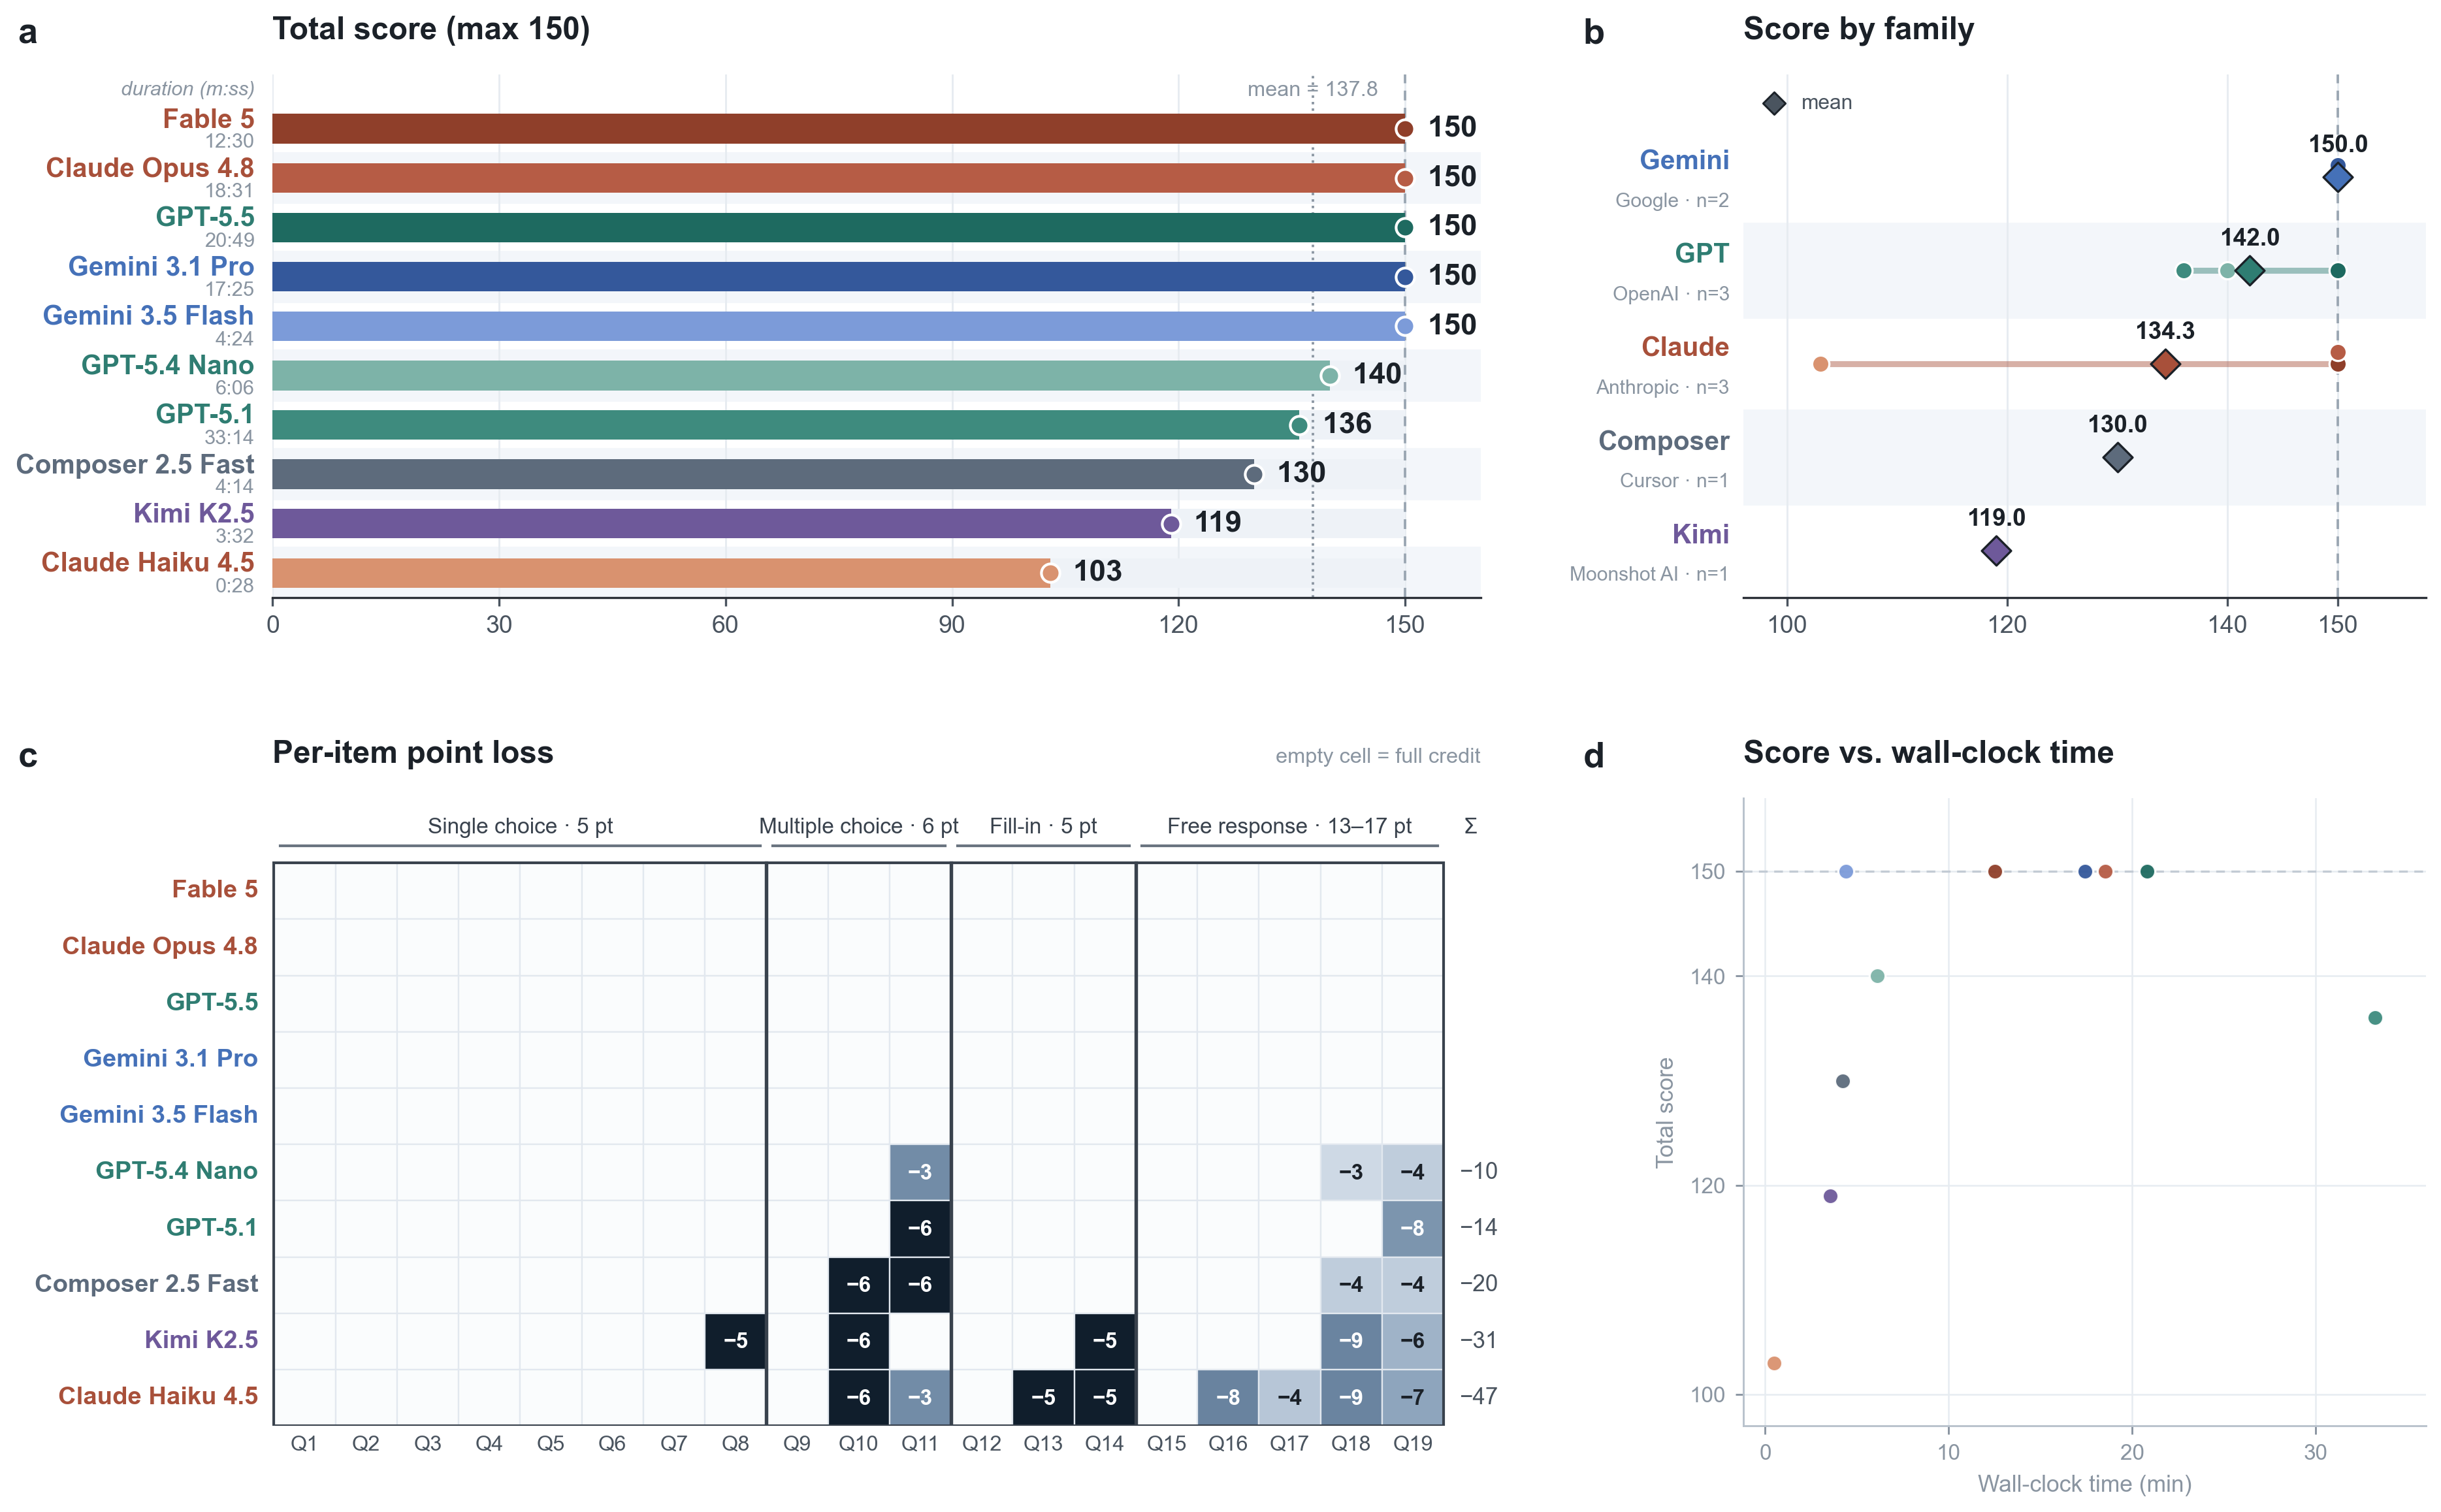
\includegraphics[width=\textwidth]{ncee2026_results_paper.png}
  \caption{Results overview. \textbf{(a)}~Total score per agent, hue by
    family, duration (m:ss) at left, cohort mean dotted. \textbf{(b)}~Score
    by family: per-model points, min--max range, diamond = family mean.
    \textbf{(c)}~Per-item point loss; empty cell = full credit; column
    blocks follow the four sections; $\Sigma$ = total loss.
    \textbf{(d)}~Total score versus wall-clock time. One closed-book
    submission per agent; provider defaults, reasoning effort medium where
    selectable; errata-verified key; multiple choice scored 6/3/0;
    equivalent forms accepted.}
  \label{fig:results}
\end{figure}

Table~\ref{tab:results} and Figure~\ref{fig:results} summarize the run.
Five findings carry the argument of the paper.

\paragraph{F1 --- The ceiling is the mode.}
Five of ten agents scored $150/150$; the cohort took $91.9\%$ of available
points (mean $137.8$, median $145$, s.d.\ $16.3$, range $103$--$150$).
Ten of nineteen items---\Q{1}--\Q{7}, \Q{9}, \Q{12}, \Q{15}---were
solved in full by every agent, including a 28-second run by a speed-tier
model. What dispersion remains is produced almost entirely by the
cohort's tail.

\paragraph{F2 --- Saturation crosses vendor lines.}
Family means---Gemini $150.0$ ($n{=}2$), GPT $142.0$ ($n{=}3$), Claude
$134.3$ ($n{=}3$), Composer $130.0$ ($n{=}1$), Kimi $119.0$
($n{=}1$)---order the table, but within-family spread (Claude:
$103$--$150$) exceeds every between-family gap at the top. The stable
observation is not a vendor ranking: every family that fielded more than
one configuration placed its strongest at the ceiling, and family means
are dragged below it by the cheaper or older members. The two
single-entry families scored under the ceiling and offer no within-family
contrast. With $n\le 3$ per family, these aggregates describe this
cohort, not the families.

\paragraph{F3 --- Points die where global structure is required.}
Section score rates: single choice $98.8\%$, fill-in $90.0\%$, free
response $91.4\%$, multiple choice $80.0\%$---the harshest section under
the 6/3/0 rule, where one wrong option voids the item. At item level,
\Q{19} (a functional-equation problem closed by an order-theoretic
argument) cost points for all five non-perfect agents; \Q{11} (a
three-circle chord family requiring an attainability check) for four;
\Q{18} (a conic pencil with a global angle minimum) for four; \Q{10} (a
solid-geometry configuration count) for three, each scoring zero. The
recurring failure is global structure---exhausting configurations,
certifying that an extremum is attained, closing a proof---not symbolic
computation, which this cohort has essentially solved. Proof-graded
evaluation isolated the same gap in earlier cohorts, with final answers
running far ahead of certified arguments \citep{petrov2025proof}; here
the gap survives only where the certification must be global.

\paragraph{F4 --- Derivation, not recall.}
The answer key circulating online fails independent verification on eight
conclusions (Appendix~\ref{app:errata}). Contamination has a signature: a
cohort reciting that key would reproduce its errors on precisely these
items. The signature is absent. Across $10$ submissions $\times$ $8$
contested conclusions, exactly one response coincided with a
circulated-but-erroneous value (one agent, \Q{16}(2)); every perfect
submission produced all eight verified values; and on \Q{11} the only
non-perfect agent to answer correctly also gave the verified \textsf{BCD}
rather than the circulated \textsf{BC}. The agents solve the paper. They
do not remember it.

\paragraph{F5 --- Time buys nothing.}
Wall-clock time spans $0{:}28$ to $33{:}14$ (median $9{:}18$) and bounds
score poorly: the fastest run scored $103$, the slowest $136$, and all
five perfect papers arrived between $4{:}24$ and $20{:}49$. Duration
reflects deployment---thinking budgets, speed tiers, orchestration
overhead---rather than competence; past roughly five minutes, additional
time bought no additional points.

\section{Discussion: The Last Scarcity}
\label{sec:discussion}

The findings above are local---one paper, one cohort, one June. The
claims they instantiate are not. We state them as propositions and trace
what they leave standing.

\paragraph{Instruments exhaust before they err.}
\begin{proposition}\label{prop:exhaustion}
The information a test item yields about its examinees is bounded by the
entropy of its response distribution; as the pass rate approaches one,
the bound approaches zero.
\end{proposition}
An item answered correctly by every examinee carries no information
about them: at pass rate $p$ the yield is at most $H(p)$ bits, and
$H(1)=0$ \citep{shannon1948mathematical}; its discrimination is zero
\citep{lord1980applications}; the response distribution has collapsed
to a point. By Proposition~\ref{prop:exhaustion}, ten of nineteen
items---and, for half
this cohort, the paper as a whole---have stopped measuring. What still
discriminates is the tail of the cohort, and the four items that demand
global arguments rather than computation (\Q{10}, \Q{11}, \Q{18},
\Q{19}). None of
this is a defect of the examination; for humans it remains a
well-calibrated instrument. It has not been refuted. It has been
exhausted---and saturation, not refutation, is how benchmarks die
\citep{ott2022mapping,kiela2021dynabench}.

\paragraph{What survived the collapse.}
Two facts outlast the dead items, and together they license everything
that follows. The solving is \emph{genuine}: under closed-book isolation,
on every contested conclusion, the cohort sides with independent
verification against the key circulating around it (F4)---derivation, not
leakage. And the solving is \emph{nearly free}: minutes of wall-clock
time, decoupled from score (F5). Real and cheap is the finding; the
scores themselves are merely its symptom.

\paragraph{Measurement prices scarcity.}
\begin{proposition}\label{prop:repricing}
The signaling value of a score is bounded by the counterfactual cost of
producing the underlying performance; a producer that drives this cost
toward zero within the measured range reprices every score in that
range, however difficult the test remains for the original population.
\end{proposition}
A score is a signal, and a signal is worth what it costs to produce
\citep{spence1973job}. The
examination's scores purchased trajectories because the underlying
performance was expensive: years of a finite adolescence, irreversibly
spent. That economics has now split in two. For a machine, a perfect
paper costs minutes and is reproducible on demand; within the measured
range, perfection has become a commodity, and every score in that range
collapses toward the price of an API call. The paper did not get
easier---excellence became abundant. A benchmark is a price list for
scarcity, and this one has been repriced. The failure mode is not
Goodhart's \citep{strathern1997improving}: no examinee gamed the measure;
a producer outside the calibrated population made the measured
performance abundant. What expires with it is not
mathematics but a proxy: the assumption that solving well-posed problems
under sealed conditions indexes a scarce human excellence. The proxy held
exactly as long as no other producer of solutions existed. It was an
accident of monopoly, and the monopoly has ended.

\paragraph{Meaning is causal, and therefore temporal.}
Why does a result that is real and cheap still fail to matter to the
system that produced it? Because mattering has a causal structure.
\begin{proposition}\label{prop:meaning}
A measurement outcome carries meaning for a system exactly insofar as
the system's future states counterfactually depend on it.
\end{proposition}
This is the only notion of meaning that survives operationalization: an
outcome on which nothing in a system's future depends is, for that
system, indistinguishable from noise
\citep[cf.][]{dretske1981knowledge,pearl2009causality}. And because causal consequence
propagates only through time, meaning is necessarily measured in
time---it exists only where a future remains that the outcome can still
reach. Apply the criterion to both examinees. For a human candidate the
score's causal cone is a life: years of preparation converge on it, and
a bifurcation of trajectory issues from it. For the agents the cone is
empty: parameters frozen, no state carried across runs, the system that
left the examination bit-identical to the system that entered. Had every
score been different, nothing in any of these systems would now differ.
A machine's $150$ is an outcome without a fate---a result that lands on
no one. It informs only the parties whose futures do depend on it:
researchers, institutions, the thirteen million. A benchmark, read
causally, is an instrument pointed at its makers. Machines have
outcomes; humans have fates.

\paragraph{The inventory of what remains scarce.}
\begin{relocationcor}
When the cost of solving approaches zero
(Proposition~\ref{prop:repricing}) and its outcome carries no consequence
for the producer (Proposition~\ref{prop:meaning}), signal and meaning
relocate jointly to whatever still carries cost and consequence: choosing
what to ask, deciding what counts as correct, and bearing irreversible
commitment.
\end{relocationcor}
If solving no longer carries the signal, what does? The experiment
contains its own answer, because everything in it that mattered happened
on the human side of the apparatus. \emph{Wanting}: someone had to find
this question worth asking; machines answer questions and do not yet own
any. \emph{Posing}: a national ritual had to be turned into a
machine-readable instrument. \emph{Adjudicating}: the key had to be
re-derived, the circulating answers overruled eight times, equivalence
ruled on---correctness itself was decided here, not in the submissions.
\emph{Staking}: hours of a finite life were bound to an outcome that
could have failed. Direction, formulation, judgment, commitment: these
are the capacities the saturated instrument never measured, and
abundance cannot mint them, because each is denominated in the one
currency that cannot be reissued---irreversible time. What collapsed was
the examination's selection function. What the collapse exposes is its
deeper one: the examination was never only a sieve; it was a mechanism
for converting years into commitment, and that conversion, unlike the
sieving, still occurs only in a human life.

\paragraph{What is left to do.}
Three tasks follow, in ascending order of difficulty. For
\emph{evaluation}: measure the edges, not the middle---item pools with
verifiable post-cutoff novelty
\citep{white2025livebench,balunovic2025matharena}, so that the
recall--derivation control of
F4 holds by construction; tasks scored on posing and adjudication (could
a system have found the eight errors no one told it to look for?);
instruments whose information lives where this cohort failed, in global
structure and certified extremes. The propositions are testable here:
dispersion, extinguished in solving, should reappear exactly where cost
and consequence persist. For \emph{institutions}: separate the
gate from the signal. The examination still ranks humans in the sealed
room with undiminished internal validity; what has decayed is external
validity \citep{messick1989validity}---the sealed room no longer
resembles a world in which solving
is ambient. Certify instead what stays scarce outside the room: judgment
under stakes, taste in problems, the willingness to be changed by what
one learns. For \emph{the rest of us}: stop asking whether machines can
pass our examinations. They can, at negligible cost, and that is
precisely why passing now proves so little. The question that remains is
not a solving problem, and therefore not theirs: which problems deserve
the one resource that cannot be rerun. None of this is the machines'
problem. All of it is ours.

\section{Limitations}

\begin{itemize}
  \item \textbf{Single run per agent.} No resampling; differences of a
        few points are not meaningful. Rankings describe one run.
  \item \textbf{Single scorer, with a conflict.} The scorer is itself a
        cohort member. Objective sections ($73/150$ points) are
        mechanically checkable and all reports are released; free-response
        grading still inherits one scorer's judgment.
  \item \textbf{Small convenience cohort.} Ten agents in one harness;
        this is a snapshot, not a controlled cross-vendor comparison.
  \item \textbf{Wall-clock, not model time.} Durations include
        orchestration and I/O and are not normalized for serving load or
        hardware.
  \item \textbf{Exposure window.} Stems were public for several days
        before the run. The errata control (F4) argues against recall of
        the circulating key, but prior exposure to stems or fragmentary
        solutions cannot be excluded entirely.
  \item \textbf{Self-reported metadata.} Three submissions record an
        effort level (high/max) other than the operator setting (medium).
        We preserve the records in the ledger and report the operator
        setting; agent self-description is itself imperfect.
  \item \textbf{One paper, one domain.} Nothing here measures research
        mathematics, problem-posing, or robustness off-distribution;
        bilingual stems may interact unevenly with different models.
\end{itemize}

\section{Conclusion}

This was a simple contrast---one fresh examination, ten agents, one run
each---and the examination was the vehicle, not the object. What it
carried: at the frontier tier, solving Gaokao mathematics is saturated,
genuinely (on every contested conclusion the cohort out-derives the key
circulating around it) and cheaply (minutes suffice; time buys nothing).
An instrument in that condition still prices deployment tiers; it no
longer prices the excellence it was built for, because that excellence is
no longer scarce. What remains scarce is what the instrument never
measured and abundance cannot mint: the wanting, posing, adjudicating,
and staking that surrounded the machines on the human side of the
apparatus---capacities denominated in irreversible time. None of this is
particular to the instrument: the propositions this run
instantiates---exhaustion, repricing, meaning as causal
consequence---hold for any benchmark pointed at any producer that is
cheaper than its examiners and unchanged by its result. We release every
artifact so that both the result and its obsolescence are reproducible.
Saturated, the examination stops measuring machines. It does not stop
measuring us.

\paragraph*{Data availability.}
All evaluation artifacts---bilingual stems, the errata-verified key, the
scoring rubric, and the frozen submissions and score reports---are
publicly available at
\url{https://github.com/xinhao-zheng/ncee-2026-math-agent-eval}.

\paragraph*{Code availability.}
The isolation protocol and the figure-generation code are available in
the same repository.

\paragraph*{Author contributions.}
X.Z. designed the study, transcribed and verified the instrument, ran
the evaluations, audited the circulating key, analyzed the results, and
wrote the manuscript.

\paragraph*{Competing interests.}
The author declares no competing interests.

\paragraph*{Ethics note.}
No human subjects were involved. Model and product names are used
descriptively; results reflect one run under the stated conditions and
should not be read as general capability claims.

\begin{thebibliography}{23}
\small\setlength{\itemsep}{2pt}
% Entries ordered by first citation in the text (Nature/Science numbering).

\bibitem[Cronbach and Meehl(1955)]{cronbach1955construct}
Cronbach, L.~J. and Meehl, P.~E. (1955). Construct validity in
psychological tests. \emph{Psychological Bulletin}, 52(4):281--302.

\bibitem[Carlini et~al.(2023)]{carlini2023quantifying}
Carlini, N., Ippolito, D., Jagielski, M., Lee, K., Tram\`er, F., and
Zhang, C. (2023). Quantifying memorization across neural language models.
In \emph{ICLR}. arXiv:2202.07646.

\bibitem[Zhang et~al.(2024)]{zhang2024careful}
Zhang, H., Da, J., Lee, D., et~al. (2024). A careful examination of
large language model performance on grade school arithmetic. In
\emph{NeurIPS Datasets and Benchmarks}. arXiv:2405.00332.

\bibitem[Oren et~al.(2024)]{oren2024proving}
Oren, Y., Meister, N., Chatterji, N., Ladhak, F., and Hashimoto, T.~B.
(2024). Proving test set contamination in black box language models. In
\emph{ICLR}. arXiv:2310.17623.

\bibitem[Zhong et~al.(2023)]{zhong2023agieval}
Zhong, W., Cui, R., Guo, Y., et~al. (2023). {AGIEval}: A human-centric
benchmark for evaluating foundation models. In \emph{Findings of NAACL
2024}. arXiv:2304.06364.

\bibitem[Zhang et~al.(2023)]{zhang2023gaokaobench}
Zhang, X., Li, C., Zong, Y., Ying, Z., He, L., and Qiu, X. (2023).
Evaluating the performance of large language models on {GAOKAO}
benchmark. arXiv:2305.12474.

\bibitem[Lei et~al.(2024)]{lei2024gaokaoeval}
Lei, Z., Liang, T., Hu, H., et~al. (2024). {GAOKAO-Eval}: Does high
scores truly reflect strong capabilities in {LLMs}? arXiv:2412.10056.

\bibitem[White et~al.(2025)]{white2025livebench}
White, C., Dooley, S., Roberts, M., et~al. (2025). {LiveBench}: A
challenging, contamination-limited {LLM} benchmark. In \emph{ICLR}.
arXiv:2406.19314.

\bibitem[Balunovi\'c et~al.(2025)]{balunovic2025matharena}
Balunovi\'c, M., Dekoninck, J., Petrov, I., Jovanovi\'c, N., and
Vechev, M. (2025). {MathArena}: Evaluating {LLMs} on uncontaminated math
competitions. arXiv:2505.23281.

\bibitem[Petrov et~al.(2025)]{petrov2025proof}
Petrov, I., Dekoninck, J., Baltadzhiev, L., et~al. (2025). Proof or
bluff? {Evaluating} {LLMs} on 2025 {USA} {Math} {Olympiad}.
arXiv:2503.21934.

\bibitem[Cobbe et~al.(2021)]{cobbe2021gsm8k}
Cobbe, K., Kosaraju, V., Bavarian, M., et~al. (2021). Training verifiers
to solve math word problems. arXiv:2110.14168.

\bibitem[Hendrycks et~al.(2021)]{hendrycks2021math}
Hendrycks, D., Burns, C., Kadavath, S., et~al. (2021). Measuring
mathematical problem solving with the {MATH} dataset. In \emph{NeurIPS
Datasets and Benchmarks}. arXiv:2103.03874.

\bibitem[Glazer et~al.(2024)]{glazer2024frontiermath}
Glazer, E., Erdil, E., Besiroglu, T., et~al. (2024). {FrontierMath}: A
benchmark for evaluating advanced mathematical reasoning in {AI}.
arXiv:2411.04872.

\bibitem[Phan et~al.(2025)]{phan2025hle}
Phan, L., Gatti, A., Han, Z., et~al. (2025). Humanity's last exam.
arXiv:2501.14249.

\bibitem[Shannon(1948)]{shannon1948mathematical}
Shannon, C.~E. (1948). A mathematical theory of communication.
\emph{Bell System Technical Journal}, 27:379--423, 623--656.

\bibitem[Lord(1980)]{lord1980applications}
Lord, F.~M. (1980). \emph{Applications of Item Response Theory to
Practical Testing Problems}. Erlbaum, Hillsdale, NJ.

\bibitem[Ott et~al.(2022)]{ott2022mapping}
Ott, S., Barbosa-Silva, A., Blagec, K., Brauner, J., and Samwald, M.
(2022). Mapping global dynamics of benchmark creation and saturation in
artificial intelligence. \emph{Nature Communications}, 13:6793.

\bibitem[Kiela et~al.(2021)]{kiela2021dynabench}
Kiela, D., Bartolo, M., Nie, Y., et~al. (2021). Dynabench: Rethinking
benchmarking in {NLP}. In \emph{NAACL}, pages 4110--4124.
arXiv:2104.14337.

\bibitem[Spence(1973)]{spence1973job}
Spence, M. (1973). Job market signaling. \emph{Quarterly Journal of
Economics}, 87(3):355--374.

\bibitem[Strathern(1997)]{strathern1997improving}
Strathern, M. (1997). `{Improving} ratings': Audit in the {British}
university system. \emph{European Review}, 5(3):305--321.

\bibitem[Dretske(1981)]{dretske1981knowledge}
Dretske, F.~I. (1981). \emph{Knowledge and the Flow of Information}.
MIT Press, Cambridge, MA.

\bibitem[Pearl(2009)]{pearl2009causality}
Pearl, J. (2009). \emph{Causality: Models, Reasoning, and Inference}.
2nd edition. Cambridge University Press.

\bibitem[Messick(1989)]{messick1989validity}
Messick, S. (1989). Validity. In Linn, R.~L., editor, \emph{Educational
Measurement}, 3rd edition, pages 13--103. American Council on
Education and Macmillan.

\end{thebibliography}

\appendix

\section{Errata to the Circulating Answer Key}
\label{app:errata}

All nineteen items were re-derived independently of the answer key
circulating online at the time of evaluation; we treat no circulating key
as authoritative. The eight circulated conclusions below fail
verification. Verified values governed scoring; circulated variants
earned no credit.

\begin{table}[h]
  \centering\small
  \caption{Circulated conclusions that fail verification.}
  \label{tab:errata}
  \begin{tabular}{@{}clll@{}}
    \toprule
    Item & Circulated & Verified & Cause of the circulated error \\
    \midrule
    \Q{11}      & \textsf{BC} & \textsf{BCD} &
      D is attained: $S_{\max}=\frac{2\sqrt{21}}{3}$ at $k^2=\frac{17}{4}$ \\
    \Q{14}      & $4$ & $\frac{\sqrt[3]{12}}{2}$ &
      sum condition misread as holding for all $n$ \\
    \Q{15}(2)   & $\frac{\sqrt{2}}{2}$ & $1$ &
      $E$ taken as midpoint of $AC$ instead of $AC_1$ \\
    \Q{16}(1)   & $\frac{\sqrt{7}}{3}$ & $\frac{1}{3}$ &
      dropped factor $2$ in $\sin A$; also $BC>AC\Rightarrow\cos A<\cos B$ \\
    \Q{16}(2)   & $\sqrt{6}$ & $3\sqrt{5}$ &
      propagates from \Q{16}(1) \\
    \Q{18}(2)(i)  & $y=\frac{1}{2}(x+1)$ & $y=\frac{\sqrt{5}}{2}(x+1)$ &
      slope of $PO$ conflated with $k$ \\
    \Q{18}(2)(ii) & $\frac{\sqrt{2}}{2}$ & $4\sqrt{3}$ &
      $PR$ is a central chord; $\angle PQR$ stays near $90^\circ$ \\
    \Q{19}(1)   & $\left(-1,\frac{3}{2}\right)$ & $\left(0,\frac{3}{2}\right)$ &
      $2^{-1+d}\le\frac{1}{2}$ misjudged on $(-1,0]$ \\
    \bottomrule
  \end{tabular}
\end{table}

Across the ten submissions, exactly one response coincided with a
circulated value above (one agent, \Q{16}(2)); every other response on
these eight conclusions either matched the verified value or matched
neither.

\end{document}
